\documentclass[times, utf8, diplomski]{fer}
\usepackage{booktabs}
\usepackage{pdfpages}
\usepackage{catchfile}
\usepackage{xparse}

% environment setup
\ExplSyntaxOn
\NewDocumentCommand{\getenv}{om}
 {
  \sys_get_shell:nnN { kpsewhich ~ --var-value ~ #2 } { } \l_tmpa_tl
  \tl_trim_spaces:N \l_tmpa_tl
  \IfNoValueTF { #1 }
   {
    \tl_use:N \l_tmpa_tl
   }
   {
    \tl_set_eq:NN #1 \l_tmpa_tl
   }
 }
\ExplSyntaxOff

\getenv[\resdir]{THESIS_RESDIR}
% done

\begin{document}
\thesisnumber{000}

\title{Naslov}

\author{Petar Mihalj}

\maketitle

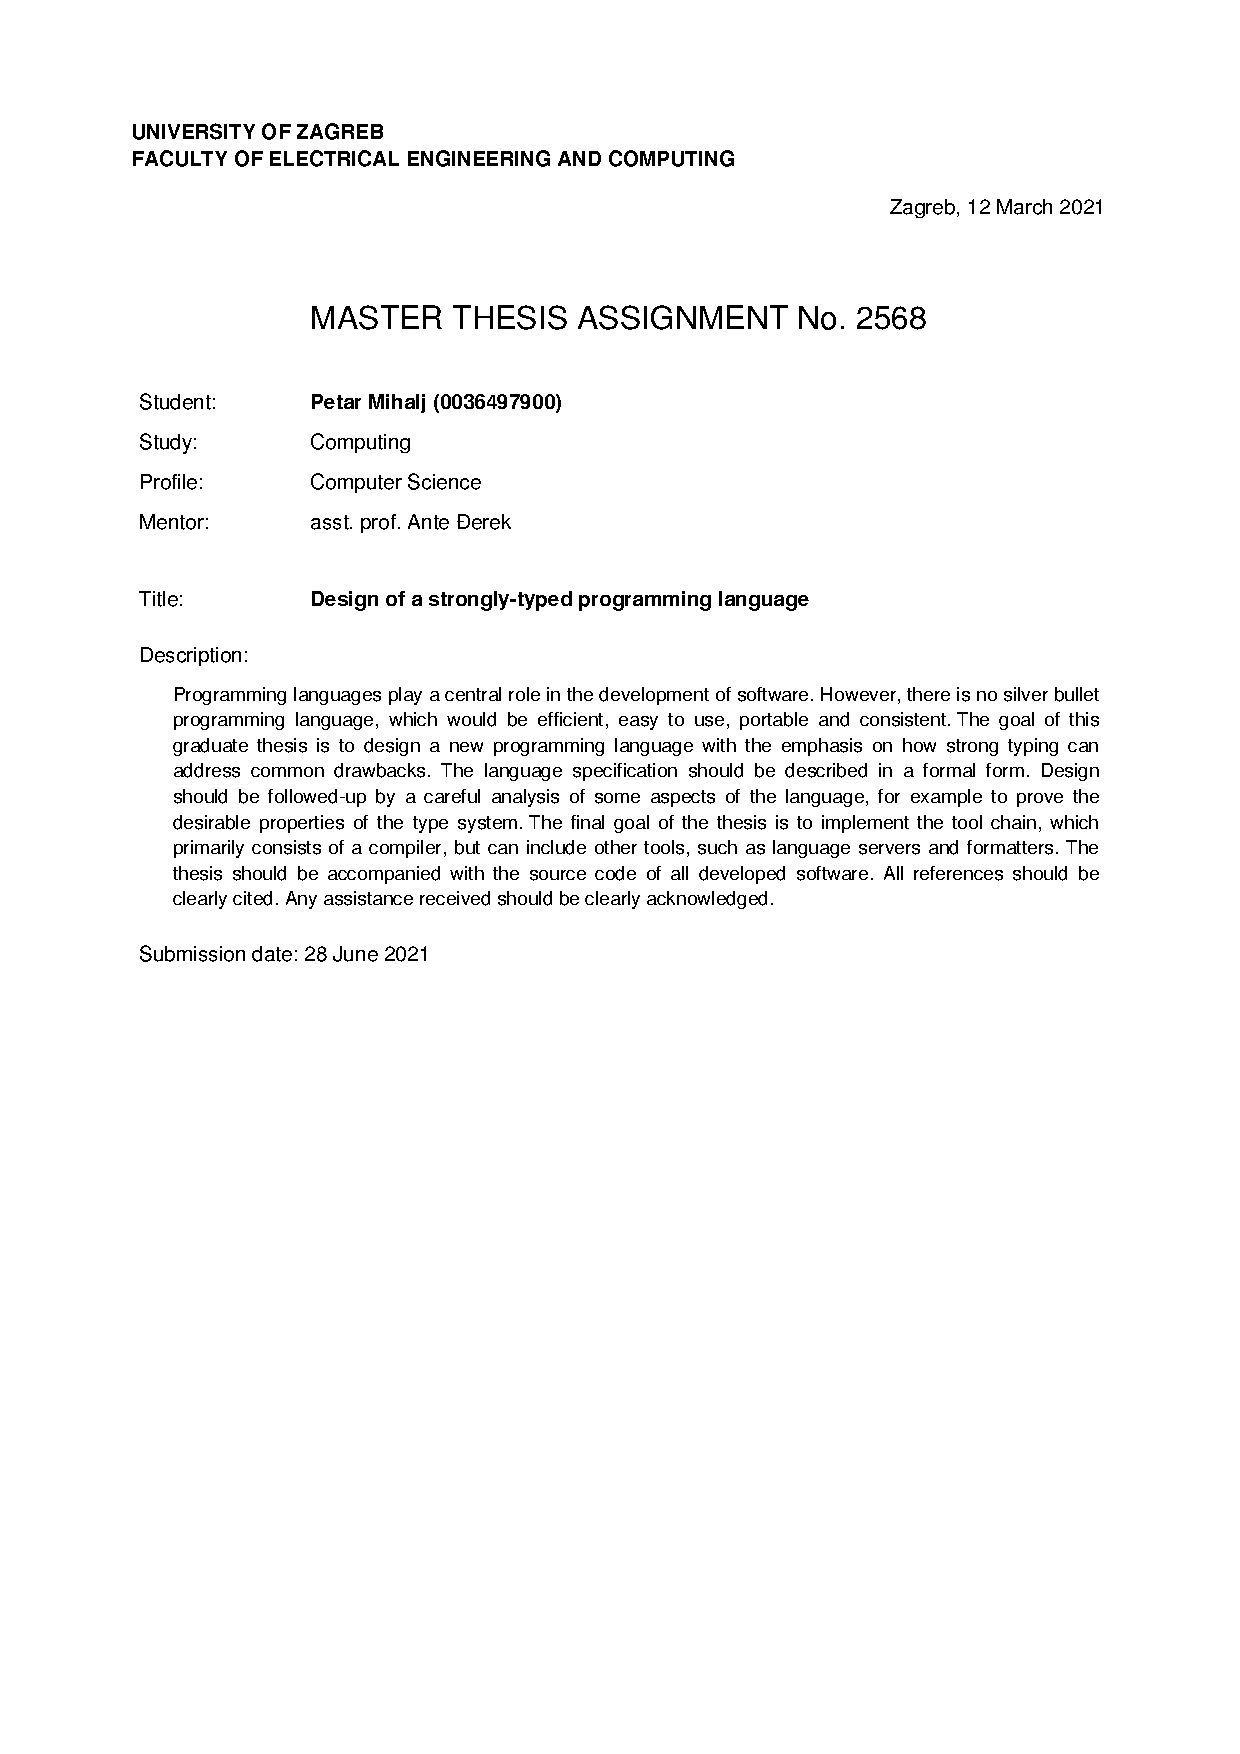
\includepdf[pages={1,2}]{\resdir/task.pdf}

\zahvala{Zahhvaljju}

\tableofcontents

\chapter{Uvod}
Uvod rada. Nakon uvoda dolaze poglavlja u kojima se obrađuje tema.
\citep{ungar2002uvod}

\chapter{Zaključak}
Zaključak.

\bibliographystyle{dinat}
\bibliography{literatura}

\begin{sazetak}
Sažetak na hrvatskom jeziku.

\kljucnerijeci{Ključne riječi, odvojene zarezima.}
\end{sazetak}

% TODO: Navedite naslov na engleskom jeziku.
\engtitle{Title}
\begin{abstract}
Abstract.

\keywords{Keywords.}
\end{abstract}

\end{document}
